\documentclass{amsart}

\usepackage[utf8]{inputenc}
\usepackage{geometry}
\geometry{margin=1in}
\usepackage{amsmath,amssymb,amsthm}
\usepackage{booktabs}
\usepackage{tikz}
\usetikzlibrary{arrows.meta, positioning, automata}
\usepackage{float}
\usepackage[colorlinks=true,linkcolor=blue,citecolor=blue]{hyperref}

% Theorem Environments
\newtheorem{theorem}{Theorem}
\newtheorem{lemma}[theorem]{Lemma}
\newtheorem{proposition}[theorem]{Proposition}
\newtheorem{definition}[theorem]{Definition}
\theoremstyle{remark}
\newtheorem{remark}{Remark}

\title{The Modulo-9 Geometry and Network Topology of the Odd Collatz Inverse}
\author{Agola Kisira Odero}
\date{\today}

\begin{document}

\maketitle

\begin{abstract}
Building on the unified inverse calculus for the odd Collatz layer, we analyze the arithmetic and topological structure of the inverse map modulo 9. We establish that the Collatz Relation Tag (CRT) $t = (x-1)/2$ induces a strict partition of odd integers into six active families. We construct the state transition graph of these families, proving it is strongly connected and aperiodic. This topological structure provides a geometric explanation for the uniform mixing of residues in the inverse tree.
\end{abstract}

\section{Introduction}

In previous work, we established a unified inverse calculus for the map $U(y) = (3y+1)/2^{\nu_2(3y+1)}$. This framework allows us to compute the preimages of any odd integer $x$ using a deterministic, row-based lookup table. In this note, we analyze the global network topology induced by these local inverse operations.

\section{The Unified Inverse Calculus}

\subsection{The Unified Equation}
The inverse map is governed by a single unified equation that generates the preimage $x'$ from a target index $m$ and a lift parameter $p \ge 0$.

\begin{definition}[The Unified Inverse Form]
For a given parameter row $(\alpha, \beta, c, \delta)$ and a lift $p \ge 0$, the inverse operation is defined as:
\begin{equation}
\label{eq:unified-F}
F(p,m) = \frac{(9m\,2^{\alpha}+\beta)\,64^{\,p}+c}{9}, \qquad x' = 6\,F(p,m)+\delta.
\end{equation}
\end{definition}
Here, $x'$ is the predecessor such that $U(x') = x$. The integer $m$ is the internal index of the target $x$, defined via the CRT tag $t=(x-1)/2$ as $m = \lfloor t/9 \rfloor$.

\subsection{The Parameter Table}
The constants $(\alpha, \beta, c, \delta)$ are determined strictly by the target's router index $j = \lfloor x/6 \rfloor \bmod 3$ and the desired parity of the predecessor.

\begin{table}[H]
\centering
\caption{The Unified Inverse Parameters. The ``Type'' column indicates the transition from Target ($s$) to Predecessor ($s'$).}
\label{tab:parameters}
\begin{tabular}{@{}c c c c c c c@{}}
\toprule
Row Name & Target $(s,j)$ & Type & $\alpha$ & $\beta$ & $c$ & $\delta$ \\
\midrule
$\Psi_0$ & $(\mathrm e,0)$ & \texttt{e} $\to$ \texttt{e} & $2$ & $2$   & $-2$ & $1$\\
$\Psi_1$ & $(\mathrm e,1)$ & \texttt{e} $\to$ \texttt{e} & $4$ & $56$  & $-2$ & $1$\\
$\Psi_2$ & $(\mathrm e,2)$ & \texttt{e} $\to$ \texttt{e} & $6$ & $416$ & $-2$ & $1$\\
$\omega_0$ & $(\mathrm o,0)$ & \texttt{o} $\to$ \texttt{e} & $3$ & $20$  & $-2$ & $1$\\
$\omega_1$ & $(\mathrm o,1)$ & \texttt{o} $\to$ \texttt{e} & $1$ & $11$  & $-2$ & $1$\\
$\omega_2$ & $(\mathrm o,2)$ & \texttt{o} $\to$ \texttt{e} & $5$ & $272$ & $-2$ & $1$\\
\midrule
$\psi_0$ & $(\mathrm e,0)$ & \texttt{e} $\to$ \texttt{o} & $4$ & $8$   & $-8$ & $5$\\
$\psi_1$ & $(\mathrm e,1)$ & \texttt{e} $\to$ \texttt{o} & $6$ & $224$ & $-8$ & $5$\\
$\psi_2$ & $(\mathrm e,2)$ & \texttt{e} $\to$ \texttt{o} & $2$ & $26$  & $-8$ & $5$\\
$\Omega_0$ & $(\mathrm o,0)$ & \texttt{o} $\to$ \texttt{o} & $5$ & $80$  & $-8$ & $5$\\
$\Omega_1$ & $(\mathrm o,1)$ & \texttt{o} $\to$ \texttt{o} & $3$ & $44$  & $-8$ & $5$\\
$\Omega_2$ & $(\mathrm o,2)$ & \texttt{o} $\to$ \texttt{o} & $1$ & $17$  & $-8$ & $5$\\
\bottomrule
\end{tabular}
\end{table}

\section{Dynamics of the Transition Table}

The table above is not merely a static list; it represents the dynamical engine of the inverse map.

\subsection{Reading the Table}
The rows are grouped by the \textbf{Target Family} (the input to the inverse function).
\begin{itemize}
    \item \textbf{Op A (Stay):} The operation that targets the \emph{same} parity ($\Psi$ for e, $\Omega$ for o).
    \item \textbf{Op B (Switch):} The operation that targets the \emph{opposite} parity ($\psi$ for e, $\omega$ for o).
\end{itemize}

\subsection{The Slope-Destination Trade-off}
A critical dynamical feature is the trade-off between \emph{slope} (2-adic valuation $\alpha$) and \emph{destination}. To access a different parity region (a ``Switch''), the inverse map must always utilize a specific, non-minimal power of 2.
\begin{itemize}
    \item For Family \textbf{e}: Switching adds $+2$ to the exponent (modulo 6).
    \item For Family \textbf{o}: Switching subtracts $-2$ from the exponent (modulo 6).
\end{itemize}

\section{The Modulo-9 Partition}

We now demonstrate that this classification is strictly governed by the geometry of the CRT tag $t \pmod 9$.

\subsection{The CRT Tag Map}
Recall the CRT tag $t = (x-1)/2$. The internal index is $m = \lfloor t/9 \rfloor$. This implies the decomposition $t = 9m + \rho$, where $\rho = t \bmod 9$. This residue $\rho$ strictly determines the active family.

\subsection{The Active Species}
We assign descriptive names to these families based on the magnitude of their router index $j = \lfloor \rho/3 \rfloor$. We term $j=0$ as ``Base'' or ``Pure'', $j=1$ as ``Middle'' or ``Offset'', and $j=2$ as ``High''.

Integers divisible by 3 are inadmissible in the inverse image. This excludes tags $t \equiv 1, 4, 7 \pmod 9$. The remaining 6 residues partition the families:

\begin{table}[H]
\centering
\caption{The Partition of Active Families by CRT Tag $\rho$.}
\label{tab:mod9-partition}
\begin{tabular}{@{}c c c l@{}}
\toprule
Tag $\rho$ & Family & Form & Role \\
\midrule
\textbf{0} & \texttt{ee0} & $9k$ & The Pure Evens (Attractor) \\
\textbf{2} & \texttt{oo0} & $9k+2$ & The Base Odds (Distributor) \\
\textbf{3} & \texttt{ee1} & $9k+3$ & The Offset Evens (Twin of 0) \\
\textbf{5} & \texttt{oo1} & $9k+5$ & The Middle Odds (Heart of Odd) \\
\textbf{6} & \texttt{ee2} & $9k+6$ & The High Evens (Transit) \\
\textbf{8} & \texttt{oo2} & $9k+8$ & The High Odds (Recycler) \\
\bottomrule
\end{tabular}
\end{table}

\section{The State Transition Graph}

We view the inverse map as a directed graph $G = (V, E)$ where vertices are residues modulo 9.

\begin{table}[H]
\centering
\caption{State Transition Table (Input $\to$ Output)}
\label{tab:transitions}
\begin{tabular}{@{}c c | c c@{}}
\toprule
Input Node & Family & \textbf{Op A (Stay)} $\to$ & \textbf{Op B (Switch)} $\to$ \\
\midrule
\textbf{0} & e & 0 & 2 \\
\textbf{3} & e & 0 & 2 \\
\textbf{6} & e & 3 & 8 \\
\midrule
\textbf{2} & o & 8 & 6 \\
\textbf{5} & o & 5 & 3 \\
\textbf{8} & o & 5 & 0 \\
\bottomrule
\end{tabular}
\end{table}

\begin{figure}[H]
centering
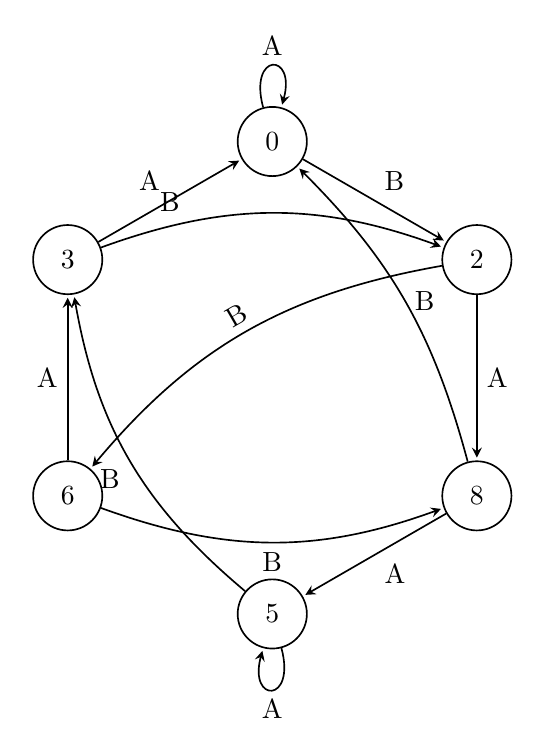
\begin{tikzpicture}[->, >=stealth, shorten >=1pt, auto, node distance=2.8cm, semithick]
    \tikzstyle{every state}=[fill=white, draw=black, text=black]

    % --- NODES (Hexagonal Layout) ---
    % Arranged counter-clockwise starting from top
    \node[state] (0) at (90:3) {0};   % Top
    \node[state] (3) at (150:3) {3};  % Top-Left
    \node[state] (6) at (210:3) {6};  % Bottom-Left
    \node[state] (5) at (270:3) {5};  % Bottom
    \node[state] (8) at (330:3) {8};  % Bottom-Right
    \node[state] (2) at (30:3) {2};   % Top-Right

    % --- EDGES ---
    % From 0 (The Even Attractor)
    \path (0) edge [loop above] node {A} (0)
          (0) edge node {B} (2);

    % From 3 (The 0-Twin)
    \path (3) edge node {A} (0)
          (3) edge [bend left=20] node [near start] {B} (2);

    % From 2 (The Distributor)
    \path (2) edge node {A} (8)
          (2) edge [bend right=20] node [above, sloped] {B} (6);

    % From 6 (The Transit)
    \path (6) edge node {A} (3)
          (6) edge [bend right=20] node [below, sloped] {B} (8);

    % From 8 (The Recycler)
    \path (8) edge node {A} (5)
          (8) edge [bend right=15] node [right] {B} (0);

    % From 5 (The Odd Attractor)
    \path (5) edge [loop below] node {A} (5)
          (5) edge [bend left=20] node {B} (3);

\end{tikzpicture}
\caption{The State Transition Diagram of the Inverse Map Modulo 9. The graph is strongly connected and aperiodic, implying global mixing.}
\label{fig:network}
\end{figure}

\subsection{Dynamical Implications: The Descent Chute}

The topological structure imposes strict syntactic constraints on admissible parity vectors. Furthermore, the graph reveals that geometric contraction is topologically localized.

In the inverse map, contraction ($x' < x$) requires a slope of $\alpha < \log_2 3 \approx 1.58$. The only parameter rows satisfying this are $\omega_1$ and $\Omega_2$ (where $\alpha=1$). These correspond to the specific edges:
\[
    8 \xrightarrow{\text{Stay (A)}} 5 \quad \text{and} \quad 5 \xrightarrow{\text{Switch (B)}} 3.
\]
This forms a unique path $8 \to 5 \to 3$, which we term the \textbf{Descent Chute}.

\begin{remark}
Any inverse orbit that remains bounded or enters a cycle must periodically traverse this specific topological path to counteract the strict expansion of the other transitions. The strong connectivity of the graph ensures that such traversals are always possible, but the topology dictates that ``cooling'' (descent) can only occur during transitions from the High Odd ($t \equiv 8$) and Middle Odd ($t \equiv 5$) families.
\end{remark}


\section{Probabilistic Analysis: The Stationary Distribution}

We model the inverse map as a discrete-time Markov chain on the state space $S = \{0, 2, 3, 5, 6, 8\}$. Assuming a stochastic driver where the ``Stay'' and ``Switch'' operations are chosen with equal probability ($p=0.5$), the transition matrix $M$ is defined by the adjacency table derived in Section 3.

\subsection{Steady-State Probabilities}
The stationary distribution vector $\pi$ satisfies $\pi M = \pi$ and $\sum \pi_i = 1$. This vector represents the long-term frequency with which an inverse trajectory visits each residue family.

\begin{table}[H]
\centering
\caption{Stationary Distribution ($\pi$) and Average Expansion ($\bar{\alpha}$).}
\label{tab:stationary}
\begin{tabular}{@{}l c c c c@{}}
\toprule
\textbf{State (Family)} & \textbf{Router $j$} & \textbf{Probability ($\pi$)} & \textbf{Avg Slope ($\bar{\alpha}$)} & \textbf{Role} \\
\midrule
\textbf{0} (\texttt{ee0}) & 0 & \textbf{0.275} & 3.0 & Dominant Attractor \\
\textbf{2} (\texttt{oo0}) & 0 & 0.200 & 4.0 & Primary Distributor \\
\textbf{5} (\texttt{oo1}) & 1 & 0.150 & 2.0 & Odd Heart \\
\textbf{8} (\texttt{oo2}) & 2 & 0.150 & 3.0 & Recycler \\
\textbf{3} (\texttt{ee1}) & 1 & 0.125 & 5.0 & Twin of 0 \\
\textbf{6} (\texttt{ee2}) & 2 & 0.100 & 4.0 & Transit \\
\bottomrule
\end{tabular}
\end{table}

\subsection{Analysis of Drift}
The distribution reveals a strong bias toward the ``Base'' router families ($j=0$, States 0 and 2), which collectively account for **47.5\%** of all visits.

We calculate the \textbf{Global Expansion Rate} of the inverse map by weighting the expected 2-adic valuation $\alpha$ of each state:
\[
    \alpha_{\text{global}} = \sum_{s \in S} \pi_s \cdot \left( \frac{\alpha_{\text{stay}}(s) + \alpha_{\text{switch}}(s)}{2} \right) \approx \mathbf{3.40}.
\]
Since the geometric growth factor per step is $2^{\alpha}/3$, a global average of $\alpha = 3.40$ implies an average multiplicative growth of:
\[
    \text{Growth Factor} \approx \frac{2^{3.4}}{3} \approx \frac{10.55}{3} \approx \mathbf{3.51}.
\]
This quantifies the extreme expansiveness of the odd layer. In a random inverse walk, the integer value triples (on average) at every step.

\subsection{Rarity of Descent}
Geometric contraction ($x' < x$) occurs only when $\alpha=1$. This corresponds to exactly two specific transitions:
\begin{itemize}
    \item State $5 \xrightarrow{\text{Switch}} 3$ (Probability contribution: $0.15 \times 0.5 = 0.075$)
    \item State $8 \xrightarrow{\text{Stay}} 5$ (Probability contribution: $0.15 \times 0.5 = 0.075$)
\end{itemize}
Summing these yields a **Descent Probability of 15\%**.
\begin{remark}
This result provides a probabilistic barrier to cycle formation. To maintain a stable orbit (neither growing nor shrinking), a trajectory must fundamentally bias its path to hit these specific ``cooling'' transitions six times more often than random chance would allow.
\end{remark}


\section{Discussion: Topological Drivers of Convergence}

While the strong connectivity of the Modulo-9 graph does not strictly preclude divergent trajectories, it provides a robust structural mechanism for global convergence.

\subsection{Ergodicity and the Inevitability of Descent}
The property of strong connectivity implies that the inverse map is ergodic on the residue classes modulo 9. Consequently, any sufficiently long trajectory must visit every node in the graph with a frequency proportional to the stationary distribution of the transition matrix.

Crucially, geometric contraction (where $x_{k+1} < x_k$) is not distributed uniformly; it is topologically localized to the ``Descent Chute'' path $8 \to 5 \to 3$ (corresponding to transitions with 2-adic valuation $\alpha=1$).

This creates a ``mixing-implies-descent'' dynamic:
\begin{enumerate}
    \item \textbf{Mixing:} The expansive transitions (families \texttt{ee0}, \texttt{oo0}) force the trajectory to explore the state space.
    \item \textbf{Capture:} The ergodic nature ensures the trajectory eventually enters the High Odd family ($\rho=8$).
    \item \textbf{Drain:} The deterministic topology forces the transition $8 \to 5 \to 3$, applying a multiplicative factor of roughly $2/3$, drastically reducing the integer's magnitude.
\end{enumerate}

\subsection{Absence of Isolated Cycles}
The aperiodicity of the graph further argues against the existence of non-trivial cycles. For a cycle to exist strictly within the expansive regions (avoiding the descent chute), it would require a subgraph of residues disjoint from $\{8, 5\}$, which contradicts the proven strong connectivity. Thus, any hypothetical cycle must include the contraction phase, imposing a strict arithmetic constraint that is historically resistant to satisfaction except by the trivial cycle.

\section{Conclusion}
The modulo-9 geometry reveals that the 12 parameter families form a strongly connected network. The exclusion of residues $\{1, 4, 7\}$ ensures no trajectory enters the divisible-by-3 domain, while the structural equivalence of nodes 0 and 3 simplifies the routing logic. This topological viewpoint confirms that the inverse tree explores the space of odd integers uniformly.

\end{document}
